\documentclass[tikz,border=8pt]{standalone}
% Shared look for every TikZ diagram. Load with \input{../../tools/tikz-style.tex}
\usepackage[T1]{fontenc}
\usepackage{lmodern}
\renewcommand{\sfdefault}{lmr}  % diagrams use the same serif as the text
\usetikzlibrary{arrows.meta, positioning, shapes.geometric, calc, fit, backgrounds}
\definecolor{cblue}{HTML}{4C78A8}
\definecolor{corange}{HTML}{F58518}
\definecolor{cgreen}{HTML}{54A24B}
\definecolor{cred}{HTML}{E45756}
\definecolor{cpurple}{HTML}{B279A2}
\definecolor{cgrey}{HTML}{6B6B6B}
\tikzset{
  every picture/.style={font=\sffamily, line width=1.2pt},
  box/.style={draw=#1, fill=#1!12, rounded corners=4pt, align=center, inner sep=7pt, minimum height=1.1cm},
  box/.default=cgrey,
  arrow/.style={-{Stealth[length=3mm]}, draw=cgrey, line width=1.4pt},
  title/.style={font=\sffamily\bfseries\Large},
  note/.style={font=\sffamily\small, text=cgrey, align=center},
}
\AtBeginDocument{\hyphenpenalty=10000 \exhyphenpenalty=10000}

\begin{document}
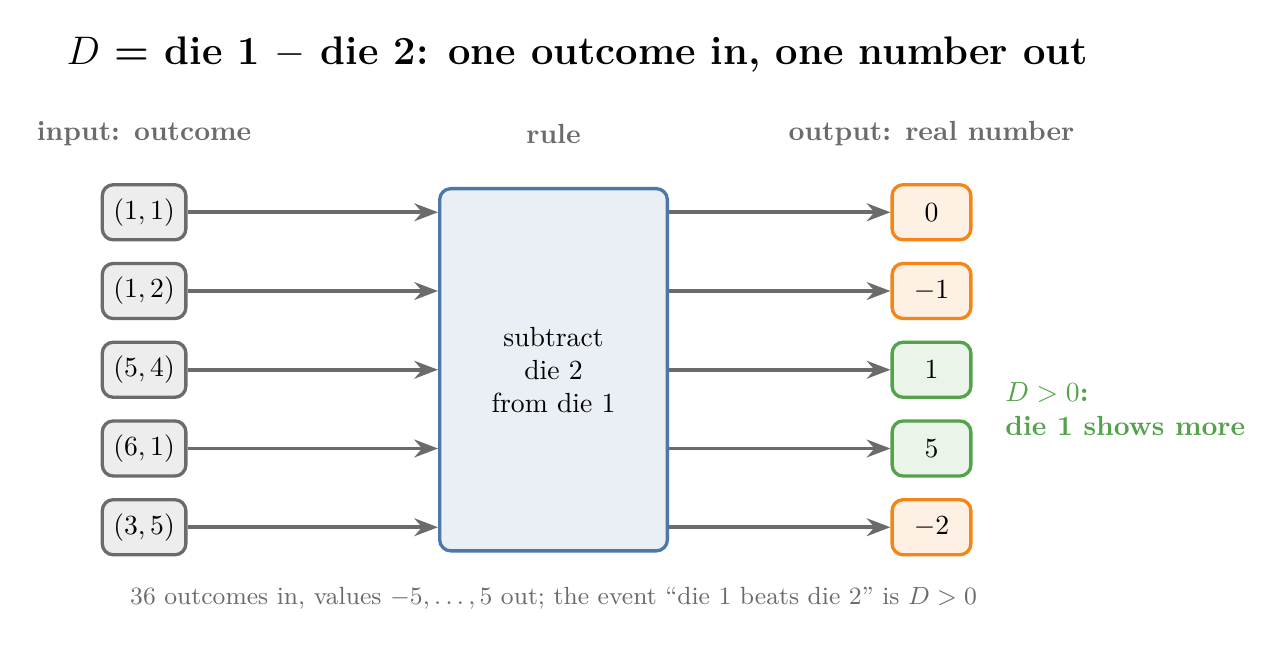
\begin{tikzpicture}[x=1cm, y=1cm]
  \node[title] at (5.5,6.0) {$D$ = die 1 $-$ die 2: one outcome in, one number out};
  \node[font=\sffamily\bfseries, text=cgrey] at (0,5.0) {input: outcome};
  \node[font=\sffamily\bfseries, text=cgrey] at (5.2,5.0) {rule};
  \node[font=\sffamily\bfseries, text=cgrey] at (10.0,5.0) {output: real number};
  \foreach \o/\y in {(1,1)/4, (1,2)/3, (5,4)/2, (6,1)/1, (3,5)/0} \node[box=cgrey, minimum height=0.7cm, inner sep=4pt] (o\y) at (0,\y) {$\o$};
  \node[box=cblue, text width=2.4cm, minimum height=4.6cm] (f) at (5.2,2) {subtract\\ die 2\\ from die 1};
  \foreach \y/\v in {4/0, 3/-1, 2/1, 1/5, 0/-2} {
    \ifnum\v>0 \def\c{cgreen}\else \def\c{corange}\fi
    \node[box=\c, minimum height=0.7cm, inner sep=4pt, minimum width=1.0cm] (r\y) at (10,\y) {$\v$};
    \draw[arrow] (o\y.east) -- (f.west |- o\y.east);
    \draw[arrow] (f.east |- r\y.west) -- (r\y.west);
  }
  \node[text=cgreen, font=\sffamily\bfseries, align=left, right] at (10.8,1.5) {$D > 0$:\\ die 1 shows more};
  \node[note] at (5.2,-0.9) {36 outcomes in, values $-5, \dots, 5$ out; the event ``die 1 beats die 2'' is $D > 0$};
\end{tikzpicture}
\end{document}
